\documentclass{article}%
\usepackage[T1]{fontenc}%
\usepackage[utf8]{inputenc}%
\usepackage{lmodern}%
\usepackage{textcomp}%
\usepackage{lastpage}%
\usepackage{authblk}%
\usepackage{graphicx}%
%
\title{Renal Overexpression of Atrial Natriuretic Peptide and Hypoxia Inducible Factor{-}1\_\_ as Adaptive Response to a High Salt Diet}%
\author{Jennifer Smith}%
\affil{Department of Pharmacology, National Medicines Institute, Warsaw, Poland}%
\date{01{-}01{-}2014}%
%
\begin{document}%
\normalsize%
\maketitle%
\section{Abstract}%
\label{sec:Abstract}%
How are these cells acting when received as part of a kidney transplant? Once controlled by dialysis and iron supplements, how can the body counter these metabolic effects that result? Learn more in a study presented here at the International Kidney Cancer Symposium (IKCS) and followed by a print presentation at the European Association for the Study of the Leukocyte (EASL) annual meeting.\newline%
Kidney deterioration as a result of kidney injury affects the health of the immune system as well as cells, and can lead to kidney stones. Recent studies have shown that DIME nanotechnology{-}based therapies may provide a treatment option to treat kidney disease and to improve progression of kidney damage. However, even when used normally, DIME causes a number of natural harmful enzymes to grow in these nephrotetic cells and those of hepatocytes, the bodys auxiliary blood cells. In reaction to this, we are able to modulate the development of these nephrotetic cells into normal cells and make them function properly in a growing blood transplant candidate.\newline%
Based on the findings of the Mature Herbs, Transplantation Transplantation (MATCH) study conducted with a live donor and a Phase 1 study of a therapeutic DIME nanotechnology{-}based treatment of Hepatitis E, in which the DIME from both recipients was administered to its two recipients, well{-}established blocking agents were employed to reverse cellular immune activation. This is in contrast to standard treatment which is involved in inducing immune rejection resulting in chronic kidney disease.\newline%
DIME nanoparticles reach targets in the skin very rapidly and generally consists of 60 nanometres of antimicrobial molecules. A two{-}minute drive to the surface of the nanomedicine triggers the metabolism of Lymphocytes, a protein that triggers activation of normalcy. This activates enzymes called phosphorylapsides to combat the presence of free radicals. Cytorylapsides activate Lymphocytes to produce more normalcy{-}producing cells such as hepatocytes. This treatment improves the establishment of normalcy in the blood and helps reverse or prevent these immune reactions.\newline%
The second study is related to a comparison of the functional outcome of the dime nano{-}sized medications with a conventional dialysis and a functional dialysis kidney in two adult nephrologists. The kidney transplant recipient and the nephrologist are operating both on dialysis and on a normal dialysis patient. Following the lymphatic system reconstructive surgery that removed tissue and the liver, the nephrologist is able to cure the kidney of injury. However, once the kidneys are restored, the biopsy of their lymph nodes results in chronic thrombocytopenia, which causes fatal white blood cell infiltration in the kidneys and has been associated with a decline in function of the central nervous system.

%
\subsection{Image Analysis}%
\label{subsec:ImageAnalysis}%


\begin{figure}[h!]%
\centering%
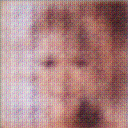
\includegraphics[width=150px]{500_fake_images/samples_5_59.png}%
\caption{A Close Up Of A Person Brushing His Teeth}%
\end{figure}

%
\end{document}